\documentclass[a4paper, 12pt]{report}
\usepackage{monapack}
\usepackage{hyperref}
\usepackage{indentfirst}
\graphicspath{{images/}}

\usepackage[outputdir=../auxil]{minted}
\usemintedstyle{friendly}

\student{Richard Kropáček}
\trida{B4.I}
\obor{18-20-M/01 Informační technologie}
\bydliste{Mírová 429, 385 01 Vimperk}
\datumNarozeni{11. 11. 2001}
\vedouci{Mgr. Milan Janoušek}
\nazevPrace{Správa povinných prací}
\cisloPrace{1}
\skolniRok{2020/2021}
\reditel{Ing. Jiří Uhlík}

\begin{document}

	\titulniStrana
	
	\anotace Výstupem mé maturitní práce je fungující systém, jehož úkolem je správa povinných prácí odevzdaných za uplynulý školní rok žáky. Učitelé
    následně mohou práce procházet, stahovat a hodnotit.\\
	\textbf{Klíčová slova: } C\#; ASP.NET Core; Entity Framework Core; HTML; JavaScript; CSS; Bootstrap; MySQL; WebApp

	\annotation The output of my graduation thesis is a functioning system, the task of which is the administration of compulsory work submitted by
    pupils for the past school year. Teachers can then browse, download and evaluate the work.\\
	\textbf{Key words: } C\#; ASP.NET Core; Entity Framework Core; HTML; JavaScript; CSS; Bootstrap; MySQL; WebApp

	\podekovani Tímto bych chtěl poděkovat Mgr. Milanu Janouškovi za vedení mé Maturitní práce, cenné rady a odborný dohled. Děkuji také za pomoc všem,
    kteří se podílěli na gramatické kontrole práce.
	
	\obsah
	
	\kapitola{Úvod}
    Pro realizaci této práce jsem se rozhodl využít ASP.NET Core, což jest otevřený framework pro tvorbu webových aplikací vyvynutý společností Microsoft.
    Pro databázi jsem se rozhodl využít MySQL, což je velice rozšířený otevřený systém řízení báze dat. Webová aplikace je psána pomocí značkovacího
    jazyku HTML. Pro vizuální část stránky jsem využil Bootstrap 4.
	\kapitola{Teoretický úvod}
		\podkapitola{Programovací jazyk C\#}
        C\# je moderní, vysokoúrovňový objektově orientovaný programocí jazyk vyvinutý společností Microsoft. Jazyk C\# se řadí mezi typově bezpečné
        programovací jazyky. To~znamená, že nedovoluje provádět operace, které mohou véct k chybám. Tento jazyk umožnuje vývojářům vytvářet mnoho
        druhů zabezpečených a robusních aplikací, které běži na~platformě .NET \footnote{Vývojářská platforma pro vytváření webových, mobilních,
        desktopových, herních, IoT a dalších aplikací. Je podporovaná v systémech Windows, Linux a macOS.}.\par
        C\# je zároveň objektově orientovaný programovací jazyk orientovaný na součásti \footnote{Component-oriented programming language}. Z~toho vyplývá,
        že se zaměřuje na vytváření komponent, které jsou tvořeny často se opakujícími částmi kódu. C\# také poskytuje jazykové kontrukce pro přímou
        podporu těchto konceptů, což z něj dělá přirozený jazyk pro tvorbu a používání těchto softwarových komponent.\cite{CSharp}
		\podkapitola{Razor}
		Razor je syntaxe pro ASP.NET používaná pro tvorbu dynamických webových stránek společně s programovacím jazykem C\#. Pomocí Razor syntaxe lze
        vložit do webové stránky blok kódu, který se provede na straně serveru. Soubory využíající tuto syntaxi mají příponu .cshtml.\par
		Razor syntaxe se skládá z Razor značek, C\# a HTML. Výchozím Razor jazykem je HTML. Pro označení C\# kódu využijeme symbolem @. Tímto dojde
        k přechodu z formátu HTML do C\#. Razor vyhodnotí výrazy jazyka C\# a vykresluje je ve výstupu HTML. Kód HTML v souborech s příponou .cshtml
        se vykreslí serverem beze změny.\cite{Razor}
		\podkapitola{ASP.NET, ASP.NET CORE}
			\begin{figure}[h!]
				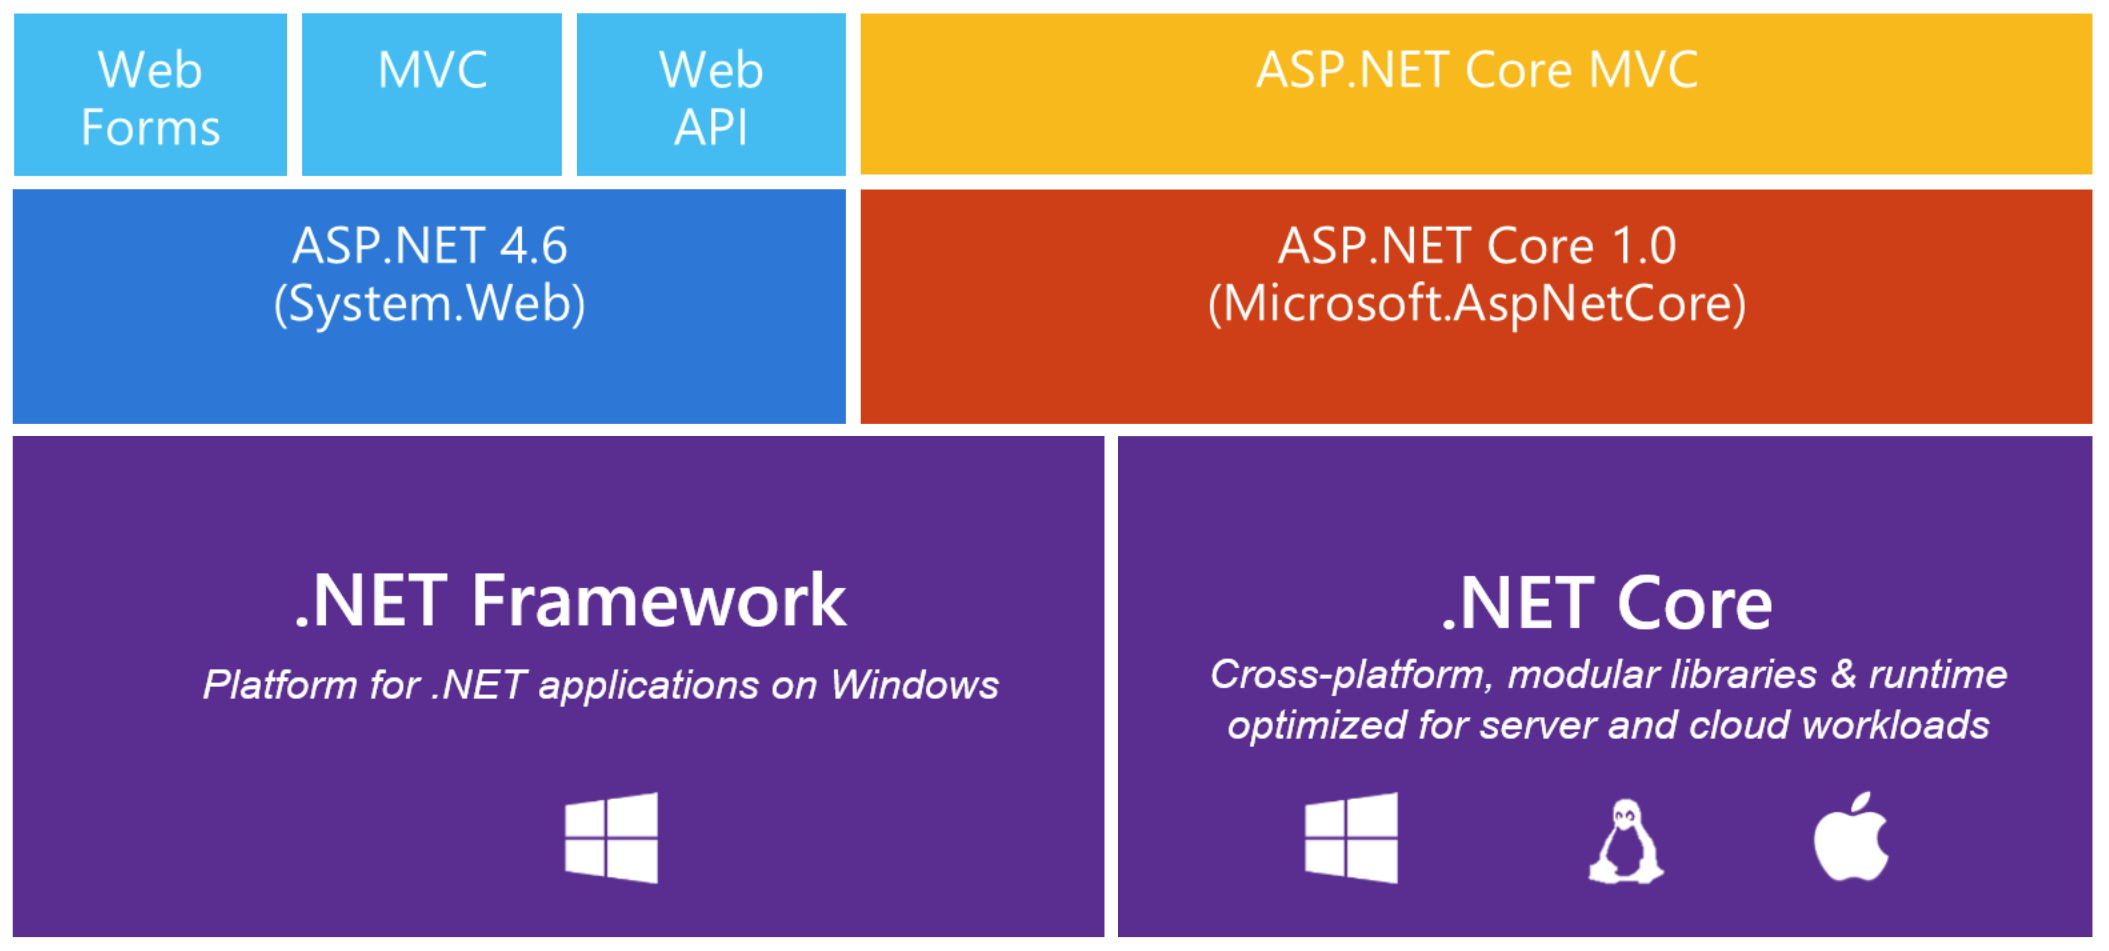
\includegraphics[width=\textwidth]{aspnetcore_aspnet}
				\caption{Porovnání ASP.NET Core a ASP.NET \cite{ASPNETCORE_ASPNET}}
				\label{ASP.NET Core a ASP.NET}
			\end{figure}
			ASP.NET je webový framework obsahující sadu knihoven, které obsahují hotová řešení mnoha základních problémů, které ve webových technologiích
            vyvstávají. Může se jednat např. o bezpečnost, autentifikaci uživatele, práci s databázemi apod.\par
			Tato technologie je založena na architektuře klient-server. Výstupem ASP.NET aplikace je HTML stránka. ASP.NET tedy běží na serveru a reaguje
            na dotazy uživatele/klienta. Pro tvorbu ASP.NET aplikace je potřeba znalost především programovacího jazyku C\# a značkovacího jazyku
            HTML.\cite{ASP.NET_Lekce1}
			\podpodkapitola{ASP.NET}
            ASP.NET je webový framework s otevřeným zdrojovým kódem, vytvořený společností Microsoft, pro vytváření moderních webových aplikací. ASP.NET
            rozšiřuje platformu .NET o nástroje a knihovny určené právě pro vytváření webových aplikací.\cite{ASP.NET}
			\podpodkapitola{ASP.NET Core}
            ASP.NET Core je open-source a multiplatformní verze ASP.NET. Tato platforma je navržena tak, aby umožnila rychlé vyvíjení runtime komponent,
            API, překladačů apod. a zároveň poskytovala stabilní a podporovanou platformu pro udržení běhu aplikací.\par
            Aplikace v ASP.NET Core lze, oproti dřívější verzi APS.NET Windows-only version, vyvíjet a spouštět v systémech Windows, Linux, macOS
            a Docker.\cite{ASP.NET_Core}

		\podkapitola{EF6 a EF Core}
        Entity Framework je Object–relational mapping (ORM) \footnote{Objektově-relační mapování}. To znamená, že se databázové tabulky přímo mapují
        na C\# třídy. V projektu následně pracujeme pouze s objekty a framework za nás na pozadí generuje SQL dotazy. Díky tomu je výsledná aplikace
        tvořena především pomocí objektů.\cite{ASP.NET_Lekce8}
			\podpodkapitola{Entity Framework 6}
            Entity Framework 6 (EF6) je ORM, primárně navržený pro .NET Framework, ale zároveň s podporou pro .NET Core. EF6 je stabilní, podporovaný
            produkt, ale již se aktivně nevyvíjí.\cite{EF6_EFCore}
			\podpodkapitola{Entity Framework Core}
				Entity Framework Core (EF Core) je moderní ORM pro .NET. Podporuje dotazy LINQ, sledování změn, aktualizace a migrace schématu.\par
				EF Core pracuje s SQL Server/SQL Azure, SQLite, Azure Cosmos DB, MySQL, PostgreSQL a mnoha dalšími druhy databází.\cite{EF6_EFCore}

		\podkapitola{MVC}
		Model-View-Controller (MVC) je návrhový vzor používaný k rozdělení webové aplikace na 3 komponenty.
		\begin{itemize}
			\item Model - Práce s daty
			\item View - Uživatelské rozhraní
			\item Controller - Logická část aplikace
		\end{itemize}\par
		Pomocí vzoru MVC pro webové aplikace jsou požadavky směrovány na controller, který je zodpovědný za práci s modelem. Model provádí akce a načítá
        data za databáze. Controller poté zvolí zobrazení (view), které se má zobrazit, a poskytne mu model. View už pouze vykreslí stránku na základě
        dat získaných z modelu.\cite{MVC}
				\podpodkapitola{Model}
				Jedná se o dynamickou datovou strukturu aplikace, nezávislou na uživatelském rozhraní. Jejím úkolem je spravovat data, pravida a logiku
                aplikace.\par
				V ASP.NET Core MVC má model podobu třídy, kde veřejné metody představují položky v databázi, s kterou je třída provázaná. Ukládáme ji
                do adresáře Models v rámci projektu. Pomocí atributů definuje pravidla, která se aplikují na klienta a server.\cite{MVC_Wiki_EN}
				\podpodkapitola{View}
				Převádí data reprezentovaná objekty modelu do podoby vhodné k interaktivní prezentaci uživateli.\cite{MVC_Wiki_CZ} Může se jednat
                o jakoukoliv reprezentaci dat (graf, diagram, tabulka, atd.).\par
				V ASP.NET Core se využívá syntaxe Razor. Ta poskytuje jednoduchý, čistý a lehký způsob vykreslení obsahu HTML stránek na základě view.
                Razor umožňuje vykreslit stránku pomocí C\# a vytvářet webové stránky plně kompatibilní s HTML5.\cite{MVC_Wiki_EN}\par
				Každý controller může pro jedno view generovat vlastní obraz. Aby tedy nedocházelo ke kolizi 2 controlleru pro jedno view, vyžaduje  MVC
                uložení view do adresáře Views v rámci projektu, a zde do podadresáře s názvem controlleru, který ho generuje (\viz{Views}).
				\begin{figure}[H]
					\centering
					\includegraphics[scale=0.7]{Views}
					\caption{Ukládání View v rámci projektu}
					\label{Views}
				\end{figure}
				\podpodkapitola{Controller}
				Controller reaguje na vstup uživatele a provádí interakce s objekty datového modelu. Zjednodušeně to znamená, že řadič přijme vstup,
                ověří jej a následně ho předá modelu.\cite{MVC_Wiki_EN}\par
				Třída controlleru obsahuje veřejné metody označené jako Action method. V ASP.NET MVC musí každý název třídy controlleru končit klíčovým
                slovem "Controller". To znamená, že pro domovské stránky třídu nazýváme HomeController, pro stránky studenta StudentController, apod.
                Všechny tyto třídy ukládáme v rámci projektu do složky Controllers.
	\begin{listing}[H]
	\begin{minted}{csharp}
	public class HomeController : Controller
	{
		public IActionResult Index()
		{
			return View();
		}
	}
	\end{minted}
	\caption{Controller - Action Method}
	\label{ActionMethod}
	\end{listing}
	\podkapitola{MySQL}
	MySQL je otevřený systém řízení báze dat uplatňující relační databázový model. Jedná se o multiplatformní databázi. Komunikace s databází probíhá
    pomocí dotazovacího jazyka SQL.\cite{MySQL_Wiki_CZ}
	\kapitola{Základní struktura ASP.NET Core}
	Pro to, aby bylo možné začít tvořit webovou aplikaci založenou na ASP.NET,
	\podkapitola{Model}
	Jak již bylo zmíněno v teorii, model se zabývá především prací s daty uloženými v databázi. Pro to, abych s nimi mohl efektivně pracovat, potřebuji
    vytvořit z jednotlivých položek databáze objekty.
	\podkapitola{View}
	\podkapitola{Controller}
		\podpodkapitola{Detail}
	\begin{listing}[H]
	\inputminted{csharp}{SourceCode/Detail.cs}
	\caption{Controller - Detail}
	\label{Detail}
	\end{listing}
		\podpodkapitola{Editace}
	\begin{listing}[H]
	\inputminted{csharp}{SourceCode/Edit.cs}
	\caption{Controller - Editace a)}
	\label{Edit}
	\end{listing}

	\begin{listing}[H]
	\inputminted{csharp}{SourceCode/Edit_Post.cs}
	\caption{Controller - Editace b)}
	\label{Edit_Post}
	\end{listing}
		\podpodkapitola{Smazání}
	\begin{listing}[H]
	\inputminted{csharp}{SourceCode/Delete.cs}
	\caption{Controller - Smazání a)}
	\label{Delete}
	\end{listing}
	\begin{listing}[H]
	\inputminted{csharp}{SourceCode/Delete_Post.cs}
	\caption{Controller - Smazání b)}
	\label{Delete_Post}
	\end{listing}
	\kapitola{Závěr}

	\seznamTabulek
	
	\seznamObrazku

	\renewcommand\listoflistingscaption{Seznam zdrojových kódů}
	\listoflistings
	

	\bibliographystyle{czechiso}
	\bibliography{main}

	\prilohy{
		\kapitola{Příloha}
	}

\end{document}